%====================================================
%
% Author: Dipl.-Inf. Xavier NOUMBISSI NOUNDOU, Ph.D. (A.B.D.)
% Email:  xnoundou7@gmail.com
%
%====================================================
\documentclass[12pt, a4paper]{article}
\NeedsTeXFormat{LaTeX2e}

%---------------------------- PACKAGE INCLUSION -------------------------------
% This group renders characters clearer and more precise

\RequirePackage[bitstream-charter,cal,expert]{mathdesign}
\RequirePackage{latexsym}

\usepackage{geometry}
\geometry{a4paper,
		  %showframe=true,
		  %margin=2.75em,
		  %a4paper,
		  %total={170mm,257mm},
		  top=3.5em,
		  left=3em,
		  right=3em,
		  bottom=3.39em
		  }

\usepackage[default]{cantarell}
\usepackage{graphicx}
\usepackage{xspace}
\usepackage[parfill]{parskip} % Activate to begin paragraphs with an empty line rather than an indent
\usepackage{paralist} % very flexible & customisable lists (eg. enumerate/itemize, etc.)
\usepackage{listings} % for lstset definitions
\usepackage{url}
\usepackage{subfig} % make it possible to include more than one captioned figure/table in a single float
\usepackage{epsfig}
\usepackage{booktabs}
%\usepackage{enumitem} %funny itemize icons
\usepackage{verbatim}
\usepackage{tcolorbox}

\usepackage{pagecolor}

\usepackage{amsmath}
\newcommand{\mathbold}[1]{\text{\textbf{#1}}}

\usepackage{xcolor}
\definecolor{yerenColorOrange}{RGB}{242, 161, 0}   
\definecolor{yerenColorBlue}{RGB}{77 , 93 , 254}
\definecolor{yerenColorRed}{RGB}{254, 48 , 48}
\definecolor{yerenColorDarkgray}{RGB}{60, 60 , 60}
\definecolor{yerenColorIndigo}{RGB}{83, 0, 125}
\definecolor{yerenColorGreen}{RGB}{2  , 160, 70}
\definecolor{forestgreen}{RGB}{2,160,70}    
\definecolor{mediumblue}{RGB}{7,43,205}    
\definecolor{firebrickred}{RGB}{178,34,34}
\definecolor{listingray}{gray}{0.9}
\definecolor{lbcolor}{rgb}{0.9,0.9,0.9}
\definecolor{darkgreen}{rgb}{0,0.35,0}
\definecolor{medgreen}{rgb}{0,0.5,0}
\definecolor{lightgreen}{rgb}{0.5,0.7,0.5}
\definecolor{pmcolour}{rgb}{0.5,0.7,0.5}
\definecolor{medgrey}{rgb}{0.6,0.6,0.6}
\definecolor{purplish}{rgb}{0.4,0,0.6}
\definecolor{brightred}{rgb}{1,0.2,0.2}

\newcommand{\diplinfn}{Dipl.--Inf.\xspace}

\newcommand{\pos}{syst\`eme--logiciel ERP\xspace}

\newcommand{\yerenlabs}{\textsc{YEROTH~R\&D}\xspace}

\newcommand{\yerenpos}{\textcolor{yerenColorBlue}{\sc YEROTH--ERP--$3.0$}\xspace}

\newcommand{\myfullacademicname}{Xavier NOUMBISSI NOUNDOU, Ph.D. (ABD)\xspace}

\usepackage{hyperref}
\hypersetup{
    colorlinks,
	pagebackref,
    citecolor=medgreen,
    linkcolor=purplish,
    breaklinks,
    pdftex,
    bookmarks,
    plainpages=false,
	pdftitle={\yerenpos, fiche~de~donn\'ees du \pos, \'edit\'ee, par: ''\myfullacademicname''},
    pdfauthor={Xavier NOUMBISSI NOUNDOU}
}

%--------------------------------------------------------------------------------

%---------------------------- COMMANDS DEFINITION -------------------------------
\newcommand{\diplinf}{\emph{Dipl.-Inf.}\xspace}

\newcommand{\emphbf}[1]{\textbf{#1}\xspace}
\newcommand{\emphit}[1]{\emph{\textit{#1}}\xspace}
\newcommand{\mycheckmark}[1]{\textcolor{#1}{$\checkmark$}\xspace}
\newcommand{\mytimes}[1]{\textcolor{#1}{$\times$}\xspace}
\newcommand{\boldsc}[1]{\textbf{\textsc{#1}}\xspace}

\newcommand{\myenumitem}[1]{\emph{#1}\xspace}
\newcommand{\yerenalert}{\emph{yeren-alert}\xspace}

\newcommand{\mysql}{MySQL\xspace}
\newcommand{\mysqlcolored}{\textcolor{yerenColorBlue}{My}\textcolor{yerenColorOrange}{SQL}\xspace}

\newcommand{\role}{r\^ole\xspace}
\newcommand{\roles}{r\^oles\xspace}

\newcommand{\manager}{<< Manager >>\xspace}
\newcommand{\magasinier}{<< Magasinier >>\xspace}
\newcommand{\caissier}{<< Caissier >>\xspace}
\newcommand{\administrateur}{<< Administrateur >>\xspace}
\newcommand{\vendeur}{<< Vendeur >>\xspace}
\newcommand{\gestionairedestocks}{<< GestionaireDesStocks >>\xspace}

\newcommand{\qt}{Qt$5$\xspace}

\newcommand{\yerenfield}[1]{\textbf{\emph{#1}}\xspace}
\newcommand{\procparagraph}[1]
	{\paragraph{ \mycheckmark{forestgreen} \emph{\textcolor{forestgreen}{#1}}}}

\newcommand{\xavier}{Xavier NOUMBISSI NOUNDOU\xspace}

\newcommand{\cmup}{\textbf{CMUP}\xspace}
\newcommand{\defdeo}{\textbf{DEF\_DEO}\xspace}
\newcommand{\fifo}{\textbf{FIFO}\xspace}
\newcommand{\lifo}{\textbf{LIFO}\xspace}

\newcommand{\featuresummary}[2]{\textbf{\textcolor{#1}{\textsc{#2}}}}

%--------------------------------------------------------------------------------

\usepackage[T1]{fontenc}
\newcommand{\changefont}[3]{
\fontfamily{#1} \fontseries{#2} \fontshape{#3} \selectfont}
\changefont{cmss}{m}{n}

% Set font to avant-garde
%\renewcommand*\rmdefault{pag}

\usepackage{fancyhdr}
\pagestyle{fancy}
\renewcommand{\headrulewidth}{0pt}
\rhead{}
\lhead{}
\cfoot{}

%Remove widows and orphants
\clubpenalty = 10000
\widowpenalty = 10000
\displaywidowpenalty = 10000

%\usepackage{fancyhdr}
%\pagestyle{fancy}
%\lhead{}
%\rhead{\bf yeren--pos--7--0@yeren.ca}

\renewcommand\labelenumi{\theenumi)}

\pagenumbering{gobble}

\begin{document}

{\bf \LARGE \yerenpos} {| \sc \scriptsize Fiche de donn\'ees du syst\`eme--logiciel }

\vspace{2.15em}

\begin{table}[!htbp]
\begin{tabular}{ll}
\parbox{27em}{

\yerenpos est un \textbf{\pos (Enterprise Resource Planing)}
qui a $6$ \textbf{types d'utilisateurs, et, r\^oles}:
\vspace{0.25em}
\begin{enumerate}
	\itemsep -0.05em
	\item \administrateur
	\item \manager
	\item \vendeur
	\item \gestionairedestocks
	\item \magasinier	
	\item \caissier.\\
\end{enumerate}

\yerenpos \textbf{a les fonctions suivantes}:
\vspace{0.25em}
\begin{enumerate}
	\itemsep -0.05em
	\item gestion des stocks
	\item alertes sur les quantit\'es en stocks,
			et sur les p\'eriodes de temps
	\item gestion des achats
	\item gestion des ventes (caisse, etc.)
	\item gestion des clients	
	\item tableaux de bord
	\item administration des utilisateurs, et, des r\^oles.\\
\end{enumerate}

\yerenpos \textbf{est}:
\vspace{0.25em}
\begin{enumerate}
	\itemsep -0.05em
	\item l\'eger, et tr\`es rapide
	\item simple, et, intuitif
	\item multi--sites (optionel).\\
\end{enumerate}

\vspace{0em}

Les tests d'utilisations de la m\'emoire sont
r\'ealis\'es avec l'outil \textbf{valgrind}.\\
}

&

\parbox{15em}{
\begin{center}
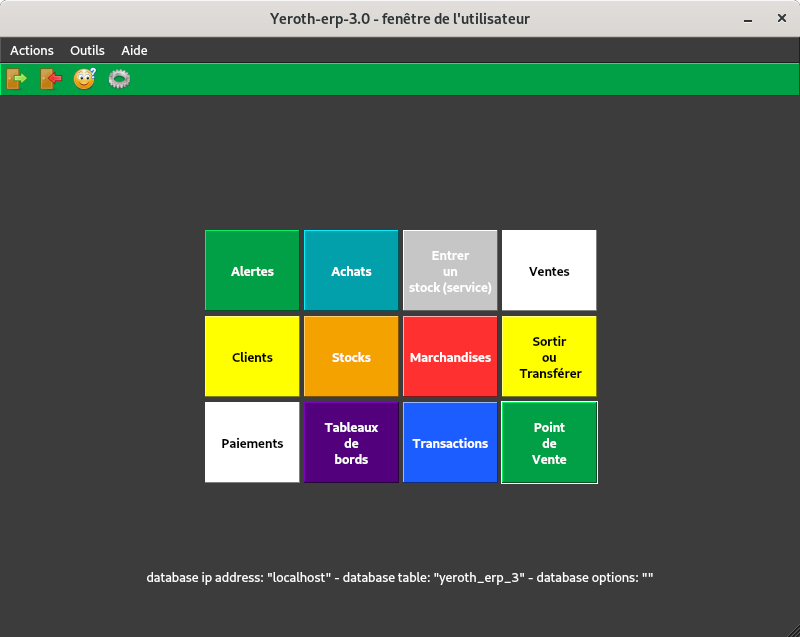
\includegraphics[scale=0.25]{images/yeroth-fenetre-manager.png}
\caption*{La fen\^etre d'acceuil pour le \manager}

\vspace{3em}

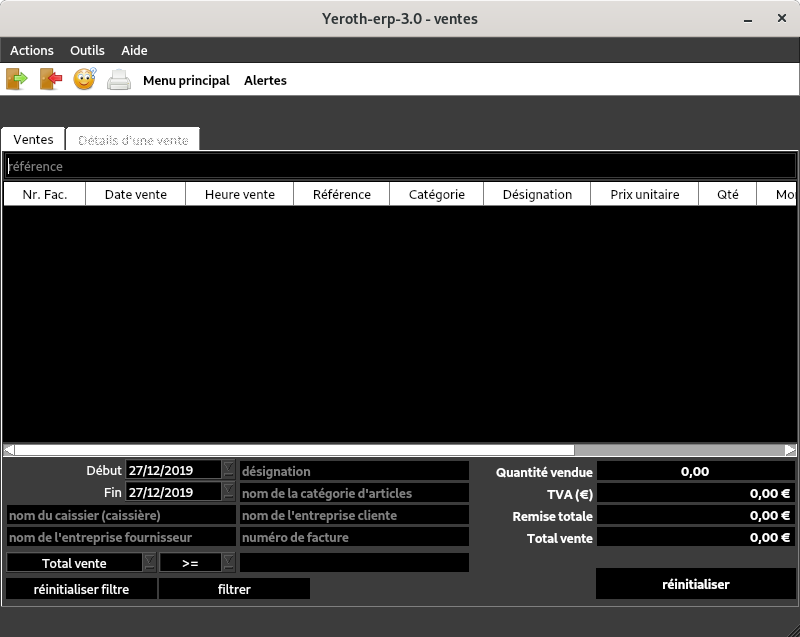
\includegraphics[scale=0.25]{images/yeroth-fenetre-caissier.png}
\caption*{La fen\^etre d'acceuil pour le \caissier}
\end{center}
}
\end{tabular}
\end{table}

\vspace{0em}

{\large \bf OP\'ERATIONS}

\vspace{0em}

\begin{table}[!htbp]
\begin{tabular}{lll}

\begin{tcolorbox}[width=14.3em, boxrule=0.01em, colback=white]
\textbf{Mat\'eriels~Point--de--Vente}
\vspace{0.1em}
\hrule
\vspace{0.25em}
\begin{itemize}[]
	\itemsep 0em
	\item[\mycheckmark{yerenColorDarkgray}] Lecteur de codes--barres, etc.\\
\end{itemize}
\begin{center}
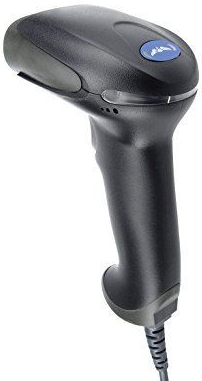
\includegraphics[scale=0.24]{images/xfox-fj-5-usb-plug-and-play-automatic-barcode-scanner.png}
\end{center}
\end{tcolorbox}

&

\begin{tcolorbox}[width=14.3em, boxrule=0.01em, colback=white]
\textbf{Syst\`emes--de--Gestion de Base--de--Donn\'ees}
\vspace{0.1em}
\hrule
\vspace{0.25em}
\begin{itemize}[]
	\itemsep 0em
	\item[\mycheckmark{yerenColorBlue}] \mysqlcolored\\
\end{itemize}
\begin{center}

\includegraphics[scale=0.164]{images/free-reuse-dbms-logo}
\end{center}
\end{tcolorbox}

&

\begin{tcolorbox}[width=14.3em, boxrule=0.01em, colback=white]
\textbf{Syst\`emes d'Exploitations}
\vspace{0.1em}
\hrule
\vspace{0.25em}
\begin{itemize}[]
	\itemsep 0em
	\item[\mycheckmark{yerenColorRed}] Windows~$10$ \& Linux--Debian\\
\end{itemize}
\begin{center}

\includegraphics[scale=0.46]{images/free-reuse-stretch-logo}
\end{center}
\end{tcolorbox}

\end{tabular}
\end{table}
	
\end{document}

